\documentclass{subfiles}

\begin{document}
\section{Time-evolution of quantum gate protocols}\label{sec:time_evolution}
We simulate the time-dependent Schrödinger equation for two distinguishable particles in our double-well Morse potential, in accordance with the procedural framework outlined in Section \ref{sec:summary_workflow}. The system is built in the Sinc-DVR basis using a grid length of $200$ a.u. with $400$ grid points, and mapped into the reduced Hartree basis as described in Section \ref{sec:Hartree_method}. We choose eigenvectors of Hamiltonian in the optimal parameters for configuration $C_I$ as our measurement (computational) basis, as the eigenvectors of this configuration have complete overlap with the logical basis states $\ket{ij}$, i.e the product states of the two particles. Our ramping protocol (Section \ref{sec:ramping_protocols}) smoothly ramps from configuration $C_I$ (non-degenerate qubit levels, zero entanglement) to configuration $C_{II}$ (close-to degeneracy in first excitations, high entanglement), and back. In what follows, we present the results of our time-evolution simulations, focusing on the state populations throughout. 

First we shall present a minimal "two-level" model of the system ($l=2$ basis functions per well) to demonstrate the idealized gate action and entanglement generation, and then we will present the full simulation ($l=4$ basis functions per well) to investigate the effects of higher-order excitations, assess higher-order leakage and its impact on gate fidelity. The discussions that follow will focus on the implications of these results for quantum control protocols and the feasibility of implementing a two-qubit gate operation in a real-world experimental setup. Time-scales in the simulations are given in atomic units (a.u.), where $1$ a.u. corresponds to approximately $2.42 \times 10^{-17}$ seconds (Hartree time), or about $58.7$ attoseconds. The total simulation times will be converted as needed to SI units, and the time steps are set to $\Delta t = 0.1$ a.u. for all simulations, ensuring a sufficiently fine resolution for capturing the dynamics of the system.

\subsection{Two-level model: Idealized gate action and entanglement generation}
In the reduced four-dimensional Hilbert space spanned by the product states $\{\ket{00}, \ket{01}, \ket{10}, \ket{11}\}$, we simulate the time evolution using the unitary time-evolution operator (Section \ref{sec:time_evolution_operator}) for the two-particle system. Because only the first four states are active, there is no possibility for population leakage to higher order states outside the qubit subspace, and we can expect the system to behave as a perfect two-qubit gate. Figure \ref{fig:time_evolution_2_basefunctions} shows the time evolution of the state populations for the two-level model, where we've plotted the populations 
\begin{align*}
    P_{ij} = |\braket{ij| \psi(t)}|^2,
\end{align*}
for each logical state $\ket{ij}$ in the qubit manifold, as a function of time.
\begin{figure}[h!]
    \centering
    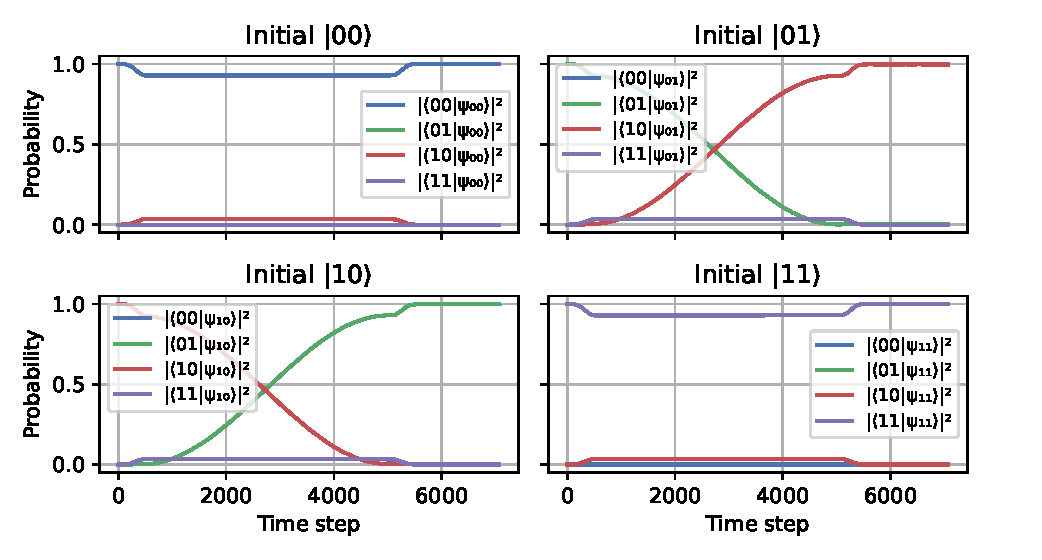
\includegraphics[width=1.0\textwidth]{figs/time_evolution_2_basefunctions_2506_SWAP.pdf}
    \caption{Evolution of the state populations for the two-level model of the Morse double-well potential using the Crank-Nicolson (CN) integrator, showing the idealized gate action and entanglement generation. The populations of the logical states $\ket{10}$ and $\ket{01}$ oscillate in a coherent manner, indicating a successful SWAP-like operation. The populations of the states $\ket{00}$ and $\ket{11}$ remain constant. The parameters used for the ramping protocol are $T_{\text{start}} = 10.0$ a.u., $T_{\text{end}} = 1500.0$ a.u, $T_{\text{up}} = 500.0$ a.u., $T_{\text{down}} = 500.0$ a.u., and the hold time $T_{\text{hold}} = 4566.0$ a.u. The ramping protocol is applied to the Morse double-well potential parameters for configuration $C_I$ and $C_{II}$, as described in Section \ref{sec:optimization_result}. The simulation is run for a total time of $T_{\text{total}} \approx 7000.0$ a.u., with a time step of $\Delta t = 0.1$ a.u. Converted using the atomic units, this corresponds to a total time $T_{\text{total}}=0.1639$ picoseconds.}
    \label{fig:time_evolution_2_basefunctions}
\end{figure}
\\ 
Parameters used to simulate the $l=2$ system are for the two configurations ($D_L, D_R, k_L, k_R, d$): $C_I = [39.9492, 40.0848, 9.4420, 8.4860, 10.3085]$ and $C_{II} = [40.0204, 41.9739, 6.9939, 7.0214, 9.9614]$. We ran a separate optimization scheme to identify these paramaters, in the same manner as for the full $l=4$ system.

Figure \ref{fig:time_evolution_2_basefunctions} shows how the populations initially is clearly separated, with clean energy eigenfunctions (e.g $\braket{\psi_0(0)|00} = 1$), before the ramping procedure is initiated at $t = 50.0$ a.u. During the ramp we see a slight nudge in the populations, where the eigenstates become populated by higher order states, that are not included in the figure. After the ramp is completed, the 1st and 2nd excited states $\psi_1(t)$ and $\psi_2(t)$, initially in $\ket{01}$ and $\ket{10}$ respectively, coherently mix. This is indication of a successful SWAP-like operation. The entanglement is generated as the populations of the two energy eigenstates mix, and swap, with a uniform frequency of oscillation $T_{\text{rabi}}$ \eqref{eq:rabi_oscillation}. This clean SWAP-like behaviour serves as a proof of concept for the two-qubit gate operation in our Morse double-well potential, demonstrating that the system can be controlled to perform a coherent SWAP of the logical states $\ket{10}$ and $\ket{01}$. At the end of the simulation the energy eigenfunctions are in a superposition, 
\begin{align*}
    \ket{\psi_1(t_{\text{end}})} &\approx 0.0027 \ket{01} + 0.9973 \ket{10}, \\
    \ket{\psi_2(t_{\text{end}})} &\approx 0.9973 \ket{01} + 0.0027 \ket{10},
\end{align*}
with negligible contributions from the states $\ket{00}$ and $\ket{11}$, which remain (almost) constant throughout the simulation. We identify the importance of optimizing the ramping procedure to ensure that the populations of the states $\ket{00}$ and $\ket{11}$ remain consistent with our desired gate operation post ramp, as the populations oscillates in time. Carefully constructed ramping protocols can be the difference between a successful (total) swap between the two states, a perfect mixing where the two states are equally populated, or a failed operation where the states go back to their original population after the gate operation has been performed. We used the Crank-Nicolson integration scheme to simulate the two-level model. \\

Qualitatively, we seem to have achieved a good SWAP gate in this simple system, and we check the gate fidelity to make a quantitative assessment of the gate operation. The logical propagator $U_{\text{logical}}$ is computed as described in Section \ref{sec:postprocessing}, and we compare it to the ideal SWAP gate \eqref{eq:swap_gate}. The classical fidelity of our gate is $F_c = 99.94\%$, while we find the average fidelity to be $F = 46.40\%$. As expected, the classical fidelity which only concerns itself with population transfer is much higher than the average fidelity. We shall see in the larger model how we can improve upon the average fidelity by clever single-qubit rotations, as explained in Section \ref{sec:postprocessing}.

\subsection{Four-level model: Higher-order excitations and gate fidelity}
In the four-level model, we include higher-order excitations by using $l=4$ basis functions per well, allowing us to investigate the effects of higher-order excitations on the gate operation, and reveal realistic limitations of the two-qubit gate operation in our Morse double-well potential. Leakage between the qubit manifold $\{\ket{01}, \ket{10}\}$ and the higher-order spectator manifolds can lead to unwanted population transfer, instability during evolution, and de-phasing effects that can significantly reduce the fidelity of the gate operation. The propagator used in the simulations are the Crank-Nicolson method, and we use the optimal parameters for the two configurations $C_I$ and $C_{II}$ as identified in Section \ref{sec:optimization_result}. We build a grid of length $200$ a.u. with $400$ grid points, and map the Sinc-DVR basis into the reduced Hartree basis with 4 functions in each well.
\subsubsection*{SWAP-gate operation}
\begin{figure}[h!]
    \centering
    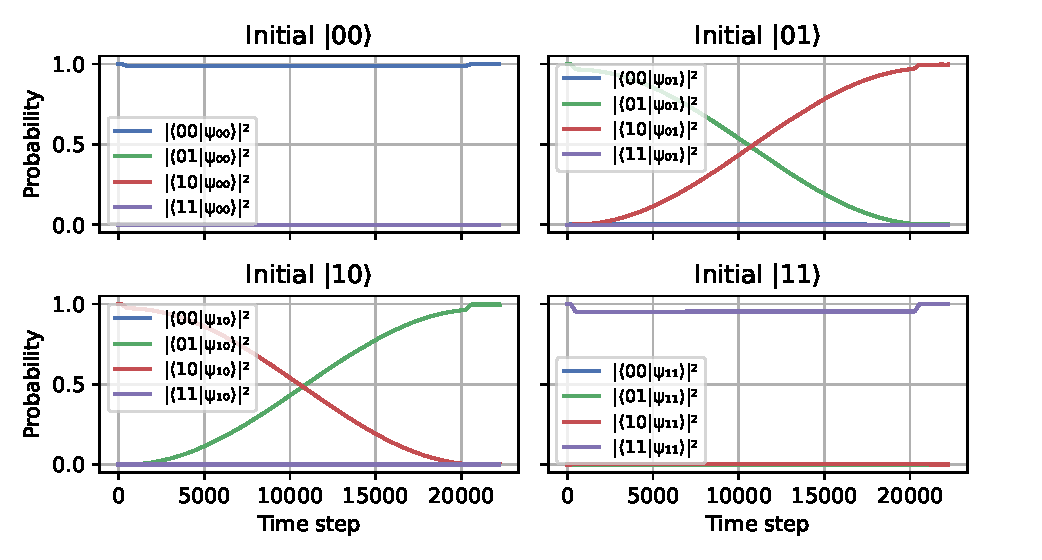
\includegraphics[width=1.0\textwidth]{figs/time_evolution_4_basefunctions_2306_SWAP.pdf}
    \caption{Evolution of the state populations for the four-level model of the Morse double-well potential using the CN integrator, showing the effects of higher-order excitations on the gate operation. The populations of the energy eigenstates $\ket{\psi_0(t)}$ and $\ket{\psi_1(t)}$ oscillate in a coherent manner, but due to the low coupling term $J=H[\psi_0, \psi_1]$ the oscillations are elongated. The coherent oscillations do indicate successful SWAP-like operation, but we note that the mixture is not clean. During evolution, there is possibly some mixture of higher order states not present in the plot.
    The parameters used in the ramping protocol are $T_{\text{start}} = 10.0$ a.u., $T_{\text{end}} = 1500.0$ a.u, $T_{\text{up}} = 500.0$ a.u., $T_{\text{down}} = 500.0$ a.u., and the hold time $T_{\text{hold}} = 19 315.0$ a.u. The ramping protocol is applied to the Morse double-well potential parameters for configuration $C_I$ and $C_{II}$, as described in Section \ref{sec:optimization_result}. The simulation is run for a total time of $T_{\text{total}} \approx 22 000.0$ a.u., with a time step of $\Delta t = 0.1$ a.u. Converted using the atomic units, this corresponds to a total time $T_{\text{total}}=0.53$ picoseconds. 
    }
    \label{fig:time_evolution_4_basefunctions}
\end{figure}
In figure \ref{fig:time_evolution_4_basefunctions} we show the time evolution of the state populations for the four-level model, where we observe similar behaviour as in the idealised two-level mode. The populations of the eigenstates $\ket{\psi_0(t)}$ and $\ket{\psi_1(t)}$ oscillate in a coherent manner, indicating a successful SWAP-like operation. The final state population of the two energy eigenstates are
\begin{align*}
    \ket{\psi_1(t_{\text{end}})} &\approx 0.9970 \ket{01} + 0.0030 \ket{10}  \\
    \ket{\psi_2(t_{\text{end}})} &\approx 0.0030 \ket{01} + 0.9970 \ket{10},
\end{align*}
and we see that we have a pure mixture of the logical states $\ket{01}$ and $\ket{10}$, and the SWAP was successful within an error of $10^{-2}$.
\\
Figure \ref{fig:time_evolution_4_basefunctions} shows the protocol with hold time to approximately match the Rabi oscillation for a successful swap of the logical states. With a coupling term of $J = 7.9674 \times 10^{-5}$ a.u., we find the Rabi oscillation \eqref{eq:rabi_oscillation} period to be $T_R = 19715 $ a.u., and we set the hold time accordingly. We note that the oscillations are elongated compared to the two-level model, indicating that the coupling term is lower than in the idealized case. This is expected, as we have higher-order excitations that can lead to leakage and de-phasing effects. 

To assess how this evolution aligns with our desired SWAP gate operation, we can compute the logical propagator $U_{\text{logical}}$,
\begin{align*}
    U_{\text{logical}} = \Psi_0^\dagger\Psi(t_f) = \begin{pmatrix}
        \braket{00|\psi_{00}(t_f)} & \braket{00|\psi_{01}(t_f)} & \braket{00|\psi_{10}(t_f)} & \braket{00|\psi_{11}(t_f)} \\
        \braket{01|\psi_{00}(t_f)} & \braket{01|\psi_{01}(t_f)} & \braket{01|\psi_{10}(t_f)} & \braket{01|\psi_{11}(t_f)} \\
        \braket{10|\psi_{00}(t_f)} & \braket{10|\psi_{01}(t_f)} & \braket{10|\psi_{10}(t_f)} & \braket{10|\psi_{11}(t_f)} \\
        \braket{11|\psi_{00}(t_f)} & \braket{11|\psi_{01}(t_f)} & \braket{11|\psi_{10}(t_f)} & \braket{11|\psi_{11}(t_f)}
    \end{pmatrix},
\end{align*}
where $\Psi(t_f)$ is the time-evolved wavefunction at the end of the simulation, and $\Psi_0$ is the initial wavefunction in the logical basis. The ideal SWAP gate operation would yield a propagator of the form \eqref{eq:swap_gate}, i.e
\begin{align*}
    U_{\text{ideal}} = \begin{pmatrix}
        1 & 0 & 0 & 0 \\
        0 & 0 & 1 & 0 \\
        0 & 1 & 0 & 0 \\
        0 & 0 & 0 & 1
    \end{pmatrix}.
\end{align*}
The result of our simulation yields the following logical propagator,
\begin{align*}
U_{\text{logical}}
=
\begin{pmatrix}
 0.7157 - 0.6984i & 0.0000 + 0.0000i & 0.0000 + 0.0000i & 0.0000 + 0.0000i \\
 0.0000 + 0.0000i & 0.0191 - 0.0518i & -0.3709 - 0.9270i & 0.0000 + 0.0000i \\
 0.0000 + 0.0000i & -0.2850 + 0.9569i & -0.0238 - 0.0498i & 0.0000 + 0.0000i \\
 0.0000 + 0.0000i & 0.0000 + 0.0000i & 0.0000 + 0.0000i & 0.9769 + 0.2135i
\end{pmatrix}
\end{align*}
and the populations of the states are given by
\begin{align*}
\lvert U_{\text{logical}}\rvert^2
=
\begin{pmatrix}
1.0000 & 0.0000 & 0.0000 & 0.0000 \\
0.0000 & 0.0030 & 0.9970 & 0.0000 \\
0.0000 & 0.9970 & 0.0030 & 0.0000 \\
0.0000 & 0.0000 & 0.0000 & 0.9998
\end{pmatrix}.
\end{align*}
We can see that the propagator is close to the ideal SWAP gate operation, with the populations of the states $\ket{00}$ and $\ket{11}$ remaining constant, while swapping the populations of the states $\ket{\psi_1}$  (initially $\ket{01}$) and $\ket{\psi_2}$ (initially $\ket{10}$) almost perfectly, to an accuracy of $99.70\%$. The small deviation can be improved upon by further optimizing the ramping protocol. We can assess the fidelity by computing the average and classical fidelity of the gate operation, equations \eqref{eq:average_fidelity} and \eqref{eq:classical_fidelity_deterministic}, respectively. The average fidelity of our gate operation is computed to be $F = 26.41\%$, using $d=4$. This indicates that while the gate operation (near) perfectly swaps the populations, it is still a no significant improvement over random operations, which would yield an average fidelity of $F = 1/d = 25\%$ \cite{zyczkowski2005average}. The deviation from the ideal SWAP gate operation arises from the fact that we do not optimize with regards to the phase evolution of the states, and instead only focus on the population transfer between the states. 

A better measurement of the gate performance as we have optimized for, would be the classical fidelity. We find the classical fidelity to be $F_c = 99.84\%$, indicating that the gate operation is indeed successful in transferring the populations of the states $\ket{01}$ and $\ket{10}$, even without much optimization of the ramping protocol, and only an approximation of the Rabi oscillation is used. By that we mean, that while we target the Rabi oscillation period exactly (to 4 decimal places), we do not account for what happens \emph{during} the parameter ramp (i.e the linear sweep between configurations), which will alter the perfect Rabi oscillation period. More studies would be needed to properly investigate the effects of the linear sweep and ramping duration on the 'perfect' Rabi oscillation period, and how this affects the gate fidelity.

\subsubsection*{$\sqrt{\text{SWAP}}$-gate operation}
In addition to the SWAP gate operation, we can also investigate the $\sqrt{\text{SWAP}}$ gate operation, which is a half-SWAP operation that transfers only half of the population from one state to another, inducing maximally entangled Bell-states\eqref{eq:bell_states} at the end of the operation. 
\begin{figure}[h!]
    \centering
    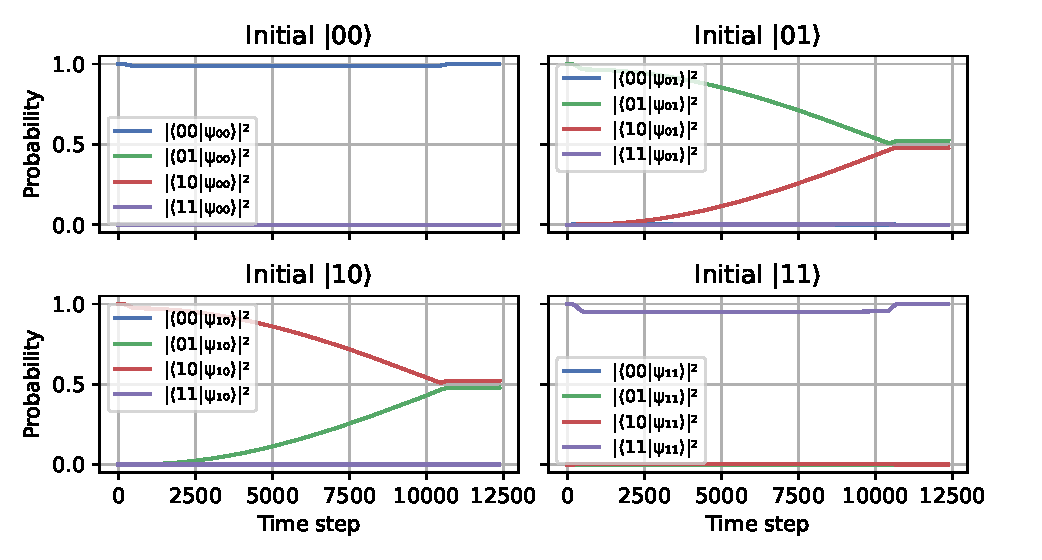
\includegraphics[width=1.0\textwidth]{figs/time_evolution_4_basefunctions_2306_squareSWAP.pdf}
    \caption{Evolution of the state populations in the four-level model of the Morse double-well potential using the CN integrator, showing the $\sqrt{\text{SWAP}}$ gate operation. The evolution is with a hold time $T_{\text{hold}} = T_{\text{SWAP}}/2 = 9857$ a.u. The ramp up and down times are set to $T_{\text{up}} = T_{\text{down}} = 500$ a.u., and we end with $T_{\text{end}} = 1500$ a.u. We see that running the evolution for a half-Swap duration results in a near-perfect mixed state, and we get Bell-like states for the first two energy eigenstates, while the remaining states remain constant. Qualitatively, this looks like we have implemented a successful $\sqrt{\text{SWAP}}$ gate-like operation, where the populations of the states $\ket{01}$ and $\ket{10}$ are mixed.}
    \label{fig:time_evolution_4_basefunctions_sqrtSWAP}
\end{figure}
Figure \ref{fig:time_evolution_4_basefunctions_sqrtSWAP} shows the time-evolution of the same system as in figure \ref{fig:time_evolution_4_basefunctions}, but with a hold time of $T_{\text{hold}} = T_{\text{SWAP}}/2 = 9857$ a.u., which is half the Rabi oscillation period. To this end, we aim to achieve a $\sqrt{\text{SWAP}}$ gate operation, which would yield a maximally entangled Bell-state at the end of the operation. Qualitatively, we see that the population of the states $\ket{01}$ and $\ket{10}$ are highly mixed, indicating that we've been successful to some degree. At the end of simulation, the populations of the two energy eigenstates are
\begin{align*}
    \ket{\psi_1(t_{\text{end}})} &\approx 0.4797 \ket{01} + 0.5203 \ket{10}, \\
    \ket{\psi_2(t_{\text{end}})} &\approx 0.5203 \ket{01} + 0.4797 \ket{10},
\end{align*}
which means we have achieved a good mixing of the two states, but not a perfect $\sqrt{\text{SWAP}}$ gate, although the states $\psi_0(t)$ and $\psi_3(t)$ remain constant (to an accuracy of $10^{-5}$). We can note that we've successfully implemented a $\sqrt{\text{SWAP}}$ gate-like operation, where the populations of the states $\ket{01}$ and $\ket{10}$ are mixed, but not to the extent that we achieve a perfect Bell-state. It is still a pure mixture (to numerical accuracy) of the two logical states $\ket{01}$ and $\ket{10}$, with no contribution from higher order states, but it is not the maximally entangled Bell-state. 
To quantitatively assess the success of the $\sqrt{\text{SWAP}}$ gate operation, we can compute the logical propagator $U_{\text{logical}}$ as before, and compare it to the ideal $\sqrt{\text{SWAP}}$ gate operation. Recall, the ideal $\sqrt{\text{SWAP}}$ \ref{eq:sqrt_swap_gate} is given by 
\begin{align*}
    U_{\sqrt{\text{SWAP}}} = \begin{pmatrix}
        1 & 0 & 0 & 0 \\
        0 & \frac{1 + i}{2} & \frac{1 - i}{2} & 0 \\
        0 & \frac{1 - i}{2} & \frac{1 + i}{2} & 0 \\
        0 & 0 & 0 & 1
    \end{pmatrix}.
\end{align*}
The result of our simulation yields
\begin{equation}
U_{\mathrm{logical}}
=
\begin{pmatrix}
 0.9635 + 0.2677i & 0.0000 + 0.0000i & 0.0000 + 0.0000i & 0.0000 + 0.0000i\\
 0.0000 + 0.0000i & 0.1459 - 0.7066i & -0.4472 - 0.5286i & 0.0000 + 0.0000i\\
 0.0000 + 0.0000i & 0.0216 + 0.6921i & -0.5814 - 0.4273i & 0.0000 + 0.0000i\\
 0.0000 + 0.0000i & 0.0000 + 0.0000i & 0.0000 + 0.0000i & -0.8709 + 0.4914i
\end{pmatrix}.
\end{equation}
Of which, if we take the element-wise modulus, we gain the population transfer matrix
\begin{equation}
\sqrt{\lvert U_{\mathrm{logical}}\rvert^2}
=\begin{pmatrix}
1.0000 & 0.0000 & 0.0000 & 0.0000\\
0.0000 & 0.7215 & 0.6924 & 0.0000\\
0.0000 & 0.6924 & 0.7215 & 0.0000\\
0.0000 & 0.0000 & 0.0000 & 1.0000
\end{pmatrix}.
\end{equation}
Calculating the gate fidelity, we find the classical fidelity to be $F_c = 73.97\%$, indicating that the gate works but is not perfect. As before, the lack of phase control throughout evolution hurts the gate fidelity, and we can improve upon this by optimizing the ramping protocol to ensure that the relative phases of the states are preserved throughout the evolution. As we are more interested in the realisation of correct population transfer, we can instead assess the fidelity of the population transfer, yielding a classical fidelity of $F_c = 99.99\%$, now calculated using \eqref{eq:classical_fidelity} due to the non-deterministic nature of the $\sqrt{\text{SWAP}}$-gate. The single-qubit rotations improved the average fidelity from $F = 25.26\%$ to $F = 77.30\%$, which is a significant improvement, but still not anywhere near the ideal $\sqrt{\text{SWAP}}$ gate operation. 

\subsubsection*{Phase correction for coherent gate fidelity}
Applying the phase correction procedure (Section \ref{sec:phase_correction}) to our raw time-evolved two-qubit unitary matrices $U_{\text{SWAP}}$ and $U_{\sqrt{\text{SWAP}}}$ dramatically improves their coherent gate fidelities. We summarize below the key numbers for both gate operations, before and after phase correction, to illustrate the impact of this procedure.
\paragraph{SWAP gate}
\begin{itemize}
    \item \textbf{Raw gate fidelity:} $F_c = 99.84\%$ (classical fidelity), $F = 26.41\%$ (average fidelity)
    \item \textbf{Optimized phase angles:} $(\theta_2, \theta_3) = (3.8832, 1.4117)$ (radians)
    \item \textbf{Phase-corrected gate fidelity:} $F_c = 99.92\%$ (classical fidelity), $F = 98.79\%$ (average fidelity)
\end{itemize}
The optimized phase angles $(\theta_2, \theta_3)$ are applied to the time-evolved unitary matrix $U_{\text{SWAP}}$, resulting in a significant increase in both classical and average fidelities. 
The optimized gate operation after phase correction is given by
\begin{equation}
G_{\mathrm{SWAP}}
=
\begin{pmatrix}
 1.0000 + 0.0000i & 0.0000 + 0.0000i & 0.0000 + 0.0000i & 0.0000 + 0.0000i\\
 0.0000 + 0.0000i & 0.0313 + 0.0455i & 0.9714 + 0.2309i & 0.0000 + 0.0000i\\
 0.0000 + 0.0000i & 0.9714 + 0.2309i & -0.0484 + 0.0265i & 0.0000 + 0.0000i\\
 0.0000 + 0.0000i & 0.0000 + 0.0000i & 0.0000 + 0.0000i & 1.0000 + 0.0000i
\end{pmatrix}.
\end{equation}
Qualitatively, this is a much better result than the raw gate operation, as the populations of the states $\ket{01}$ and $\ket{10}$ are now pure to a tolerance of $10^{-3}$, and the populations of the states $\ket{00}$ and $\ket{11}$ are now constant with no relative phase. 

\paragraph{$\sqrt{\text{SWAP}}$ gate}
\begin{itemize}
    \item \textbf{Raw gate fidelity:} $F_c = 73.97\%$ (classical fidelity), $F = 25.26\%$ (average fidelity)
    \item \textbf{Optimized phase angles:} $(\theta_2, \theta_3) = (2.8589, 1.0674)$ (radians)
    \item \textbf{Phase-corrected gate fidelity:} $F_c = 99.99\%$ (classical fidelity), $F = 77.30\%$ (average fidelity)
\end{itemize}
The optimized phase angles $(\theta_2, \theta_3)$ are applied to the time-evolved unitary matrix $U_{\sqrt{\text{SWAP}}}$, resulting in once again a significant increase in both classical and average fidelities. We are not as successful in improving the average fidelity as we were for the SWAP gate, likely due to the more complex phase factors present in the ideal gate operation.
The optimized gate matrix is given by
\begin{equation}
G_{\sqrt{\mathrm{SWAP}}}
=
\begin{pmatrix}
 1.0000 + 0.0000i & 0.0000 + 0.0000i & 0.0000 + 0.0000i & 0.0000 + 0.0000i\\
 0.0000 + 0.0000i & 0.6072 - 0.3898i & 0.0652 - 0.6893i & 0.0000 + 0.0000i\\
 0.0000 + 0.0000i & -0.3823 - 0.5773i & 0.7192 + 0.0577i & 0.0000 + 0.0000i\\
 0.0000 + 0.0000i & 0.0000 + 0.0000i & 0.0000 + 0.0000i & 1.0000 + 0.0000i
\end{pmatrix}.
\end{equation}
Qualitatively, we see that the phase correction has improved the gate operation immensively, as the populations of the states $\ket{01}$ and $\ket{10}$ are now mixed cleanly to a much higher degree, and the population of states $\ket{00}$ and $\ket{11}$ are now constant with no relative phase. There is still room for improvement, and we again would need to optimize further the ramping protocol to ensure that the relative phases of are more easily optimized by our correction procedure.

These results demonstrate the effectiveness of the phase correction procedure in improving the coherent gate fidelities of our two-qubit gate operations. Initially, our average fidelities were no better than random operations ($\approx 25\%$), but after a single phase correction step, we achieved average fidelities of $98.79\%$ for the SWAP gate and $77.30\%$ for the $\sqrt{\text{SWAP}}$ gate, with classical fidelities of $99.92\%$ and $99.99\%$, respectively. This highlights the importance of phase control in quantum gate operations, and how it can significantly enhance two-qubit operations. In exprimental setups, such single-qubit phase corrections are usually integrated into the two-qubit gate protocols \cite{nielsen2010quantum}.
\end{document}